\documentclass[aspectratio=43]{beamer}
\usepackage[english]{babel}
\usepackage{amsthm}
\usepackage{mathtools}
\usepackage{physics}
\usepackage{calligra}
\usepackage{csquotes}
\usepackage{tensor}
\usepackage[thicklines]{cancel}
\usepackage{tcolorbox}
\usepackage{pstricks}
\usepackage[backend=biber, bibstyle=nature, sorting=nty, citestyle=numeric-comp]{biblatex} %Custom bibliography
\usepackage{etoolbox}
\makeatletter
\patchcmd{\@verbatim}
{\verbatim@font}
{\verbatim@font\small}
{}{}
\makeatother
\addbibresource{bib.bib} %Load references


\DeclareMathAlphabet{\mathcalligra}{T1}{calligra}{m}{n}
\DeclareFontShape{T1}{calligra}{m}{n}{<->s*[2.2]callig15}{}
\newcommand{\scriptr}{\mathcalligra{r}\,}
\newcommand{\boldscriptr}{\pmb{\mathcalligra{r}}\,}
\def\rc{\scriptr}
\def\brc{\boldscriptr}
\def\hrc{\hat\brc}
\newcommand{\ie}{\emph{i.e.}} %id est
\newcommand{\eg}{\emph{e.g.}} %exempli gratia
\newcommand{\rtd}[1]{\ensuremath{\left\lfloor #1 \right\rfloor}}
\newcommand{\dirac}[1]{\ensuremath{\delta \left( #1 \right)}}
\newcommand{\diract}[1]{\ensuremath{\delta^3 \left( #1 \right)}}
\newcommand{\e}{\ensuremath{\epsilon_0}}
\newcommand{\m}{\ensuremath{\mu_0}}
\newcommand{\V}{\ensuremath{\mathcal{V}}}
\newcommand{\prnt}[1]{\ensuremath{\left(#1\right)}} %parentheses
\newcommand{\colch}[1]{\ensuremath{\left[#1\right]}} %square brackets
\newcommand{\chave}[1]{\ensuremath{\left\{#1\right\}}}  %curly brackets

\useoutertheme{infolines}
\useinnertheme{rectangles}
\usefonttheme{professionalfonts}


\definecolor{orange}{HTML}{f28165}
\definecolor{gray}{HTML}{303030}
\definecolor{yellow}{HTML}{f0be52}
\definecolor{lightorange}{HTML}{f19e58}

\renewcommand{\CancelColor}{\color{orange}}

\makeatletter
\newcommand{\mybox}[1]{%
	\setbox0=\hbox{#1}%
	\setlength{\@tempdima}{\dimexpr\wd0+13pt}%
	\begin{tcolorbox}[colback=orange,colframe=orange,boxrule=0.5pt,arc=4pt,
		left=6pt,right=6pt,top=6pt,bottom=6pt,boxsep=0pt,width=\@tempdima]
		\textcolor{white}{#1}
	\end{tcolorbox}
}
\makeatother

\usecolortheme[named=orange]{structure}
\usecolortheme{sidebartab}
\usecolortheme{orchid}
\usecolortheme{whale}
\setbeamercolor{alerted text}{fg=yellow}
\setbeamercolor{block title alerted}{bg=alerted text.fg!90!black}
\setbeamercolor{block title example}{bg=lightorange!60!black}
\setbeamercolor{background canvas}{bg=gray}
\setbeamercolor{normal text}{bg=gray,fg=white}

\setbeamertemplate{footline}
{
	\leavevmode%
	\hbox{%
		\begin{beamercolorbox}[wd=.333333\paperwidth,ht=2.25ex,dp=1ex,center]{author in head/foot}%
			\usebeamerfont{author in head/foot}\insertshortauthor~~(\insertshortinstitute)
		\end{beamercolorbox}%
		\begin{beamercolorbox}[wd=.333333\paperwidth,ht=2.25ex,dp=1ex,center]{title in head/foot}%
			\usebeamerfont{title in head/foot}\insertshorttitle
		\end{beamercolorbox}%
		\begin{beamercolorbox}[wd=.333333\paperwidth,ht=2.25ex,dp=1ex,center]{date in head/foot}%
			\usebeamerfont{date in head/foot}\insertframenumber/\inserttotalframenumber%\insertshortdate{}%\hspace*{2em}
			
			%#turning the next line into a comment, erases the frame numbers
			%\insertframenumber{} / \inserttotalframenumber\hspace*{2ex} 
			
	\end{beamercolorbox}}%
	\vskip0pt%
}


\setbeamertemplate{blocks}[rectangle]
\setbeamercovered{dynamic}

\setbeamertemplate{section page}
{
	\begin{centering}
		\begin{beamercolorbox}[sep=27pt,center]{part title}
			\usebeamerfont{section title}\insertsection\par
			\usebeamerfont{subsection title}\insertsubsection\par
		\end{beamercolorbox}
	\end{centering}
}

%\setbeamertemplate{subsection page}
%{
%	\begin{centering}
%		\begin{beamercolorbox}[sep=12pt,center]{part title}
%			\usebeamerfont{subsection title}\insertsubsection\par
%		\end{beamercolorbox}
%	\end{centering}
%}

\newcommand{\hlight}[1]{\colorbox{violet!50}{#1}}
\newcommand{\hlighta}[1]{\colorbox{red!50}{#1}}

\title{Final Task - Robot Server Interaction} %->->->->-> Check hyperref title <-<-<-<-<-
\subtitle{CS565 - Scientific Computing}
\author[A. Dunn \& J. Phan]{Andrew Dunn and Justin Phan}
\institute[CSCWU]{
    Department of Computer Science%
    \\%
    Central Washington University%
} %You can change the Institution if you are from somewhere else
\date{\today}
%\logo{
\includegraphics[width= 0.2\textwidth]{images/a-logo.png}}

\begin{document}
    
    \frame{\titlepage}
    
    \begin{frame}{Summary}
        \tableofcontents
    \end{frame}
    \section{Introduction}
    
    \frame{\sectionpage}
    
    \begin{frame}{Problem Description}
		\begin{itemize}
			\item Using Nao Robot to connect to our VPS server
			\pause
			\item Nao Robot uses python2 to receive random quote from our server
			\pause
			\item Nao Robot repeats quote to our audience
		\end{itemize}
	\end{frame} 
    
    \section{What software did we use?}
    
    \frame{\sectionpage}
    
    \begin{frame}{Software we used}
		\begin{itemize}
			\item ApacheSpark and Python3 on the server
			\pause
			\item Python2 on the robot
		\end{itemize}
	\end{frame}
    
    \section{Server Implementation}
 
\frame{\sectionpage}
 
\begin{frame}[fragile]{Initializing Spark DataFrame and Flask}
	\begin{verbatim}
	print("### Initializing Spark Context")
	sc, sql_ctx, spark = init_spark("Spark_Webserver", "local[4]")
	
	print("### Creating Spark dataframe from file")
	df = spark.read.json("quotes-table.json")
	
	print("### Initializing Flask app")
	app = Flask(__name__)
	\end{verbatim}
\end{frame}
	
\begin{frame}[fragile]{Using Spark to run dataframe query}
	\begin{verbatim}
	# Get author parameter from url (ex: [server-ip]/?author=tesla)
	author_arg = request.args.get('author', default = "", 
	    type = str).lower().strip()
	
	# Get all rows where author column string contains 
	# author_arg substring
	author_quotes = df.filter(
	    lower(df.author).like("%" + author_arg + "%"))
	\end{verbatim}
\end{frame}

\begin{frame}[fragile]{Using Flask to return the web request as JSON}
	\begin{verbatim}
	# Generate random number for row index
	random_row = random.randint(0, num_quotes - 1)
	
	# Collect table rows, converting that dataframe to a python list
	rows = author_quotes.collect()
	
	# Retrieve the random row's quote and author
	quote = str(rows[random_row]["quote"])
	author = str(rows[random_row]["author"])
	
	# Return response
	return '{"quote":"' + quote + '", "author":"' + author + '"}'
	\end{verbatim}
\end{frame}

\begin{frame}{Quotes database}
	\begin{figure}
		\centering
		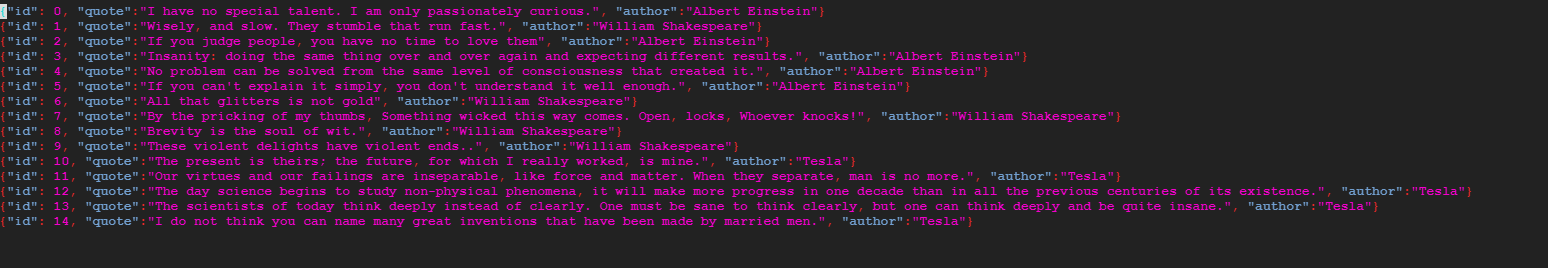
\includegraphics[width =1\linewidth]{robot-spark-proj/quotes-table.PNG}
		\caption{quotes-database.json file}
	\end{figure}
	
\end{frame}

 
    
    \section{Robot Implementation}
    
    \frame{\sectionpage}
    
    \begin{frame}{Robot program trigger phrases}
    	\begin{itemize}
    		\item "Give me a quote"
    		\item "I'd like a quote"
    		\item "Can I have a quote"
    	\end{itemize}
    \end{frame}
    
    \begin{frame}{Nao 6 Project Settings}
    	\begin{figure}
    		\centering
    		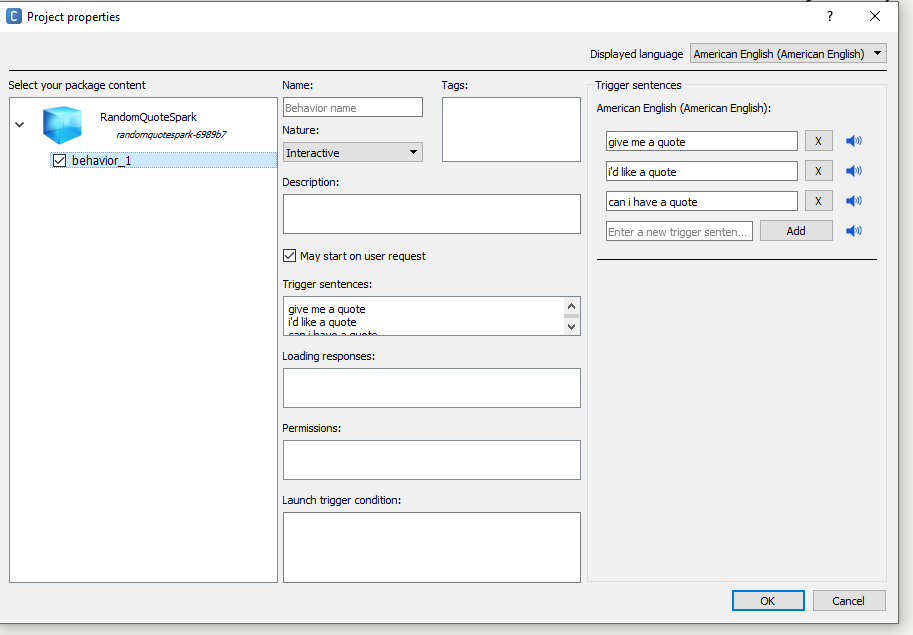
\includegraphics[width =0.7\linewidth]{robot-spark-proj/screenshot-3.PNG}
    		\caption{Robot trigger}
    	\end{figure}
    	
    \end{frame}
    
    \begin{frame}{Nao 6 Choreograph Program}
    	\begin{figure}
    		\centering
    		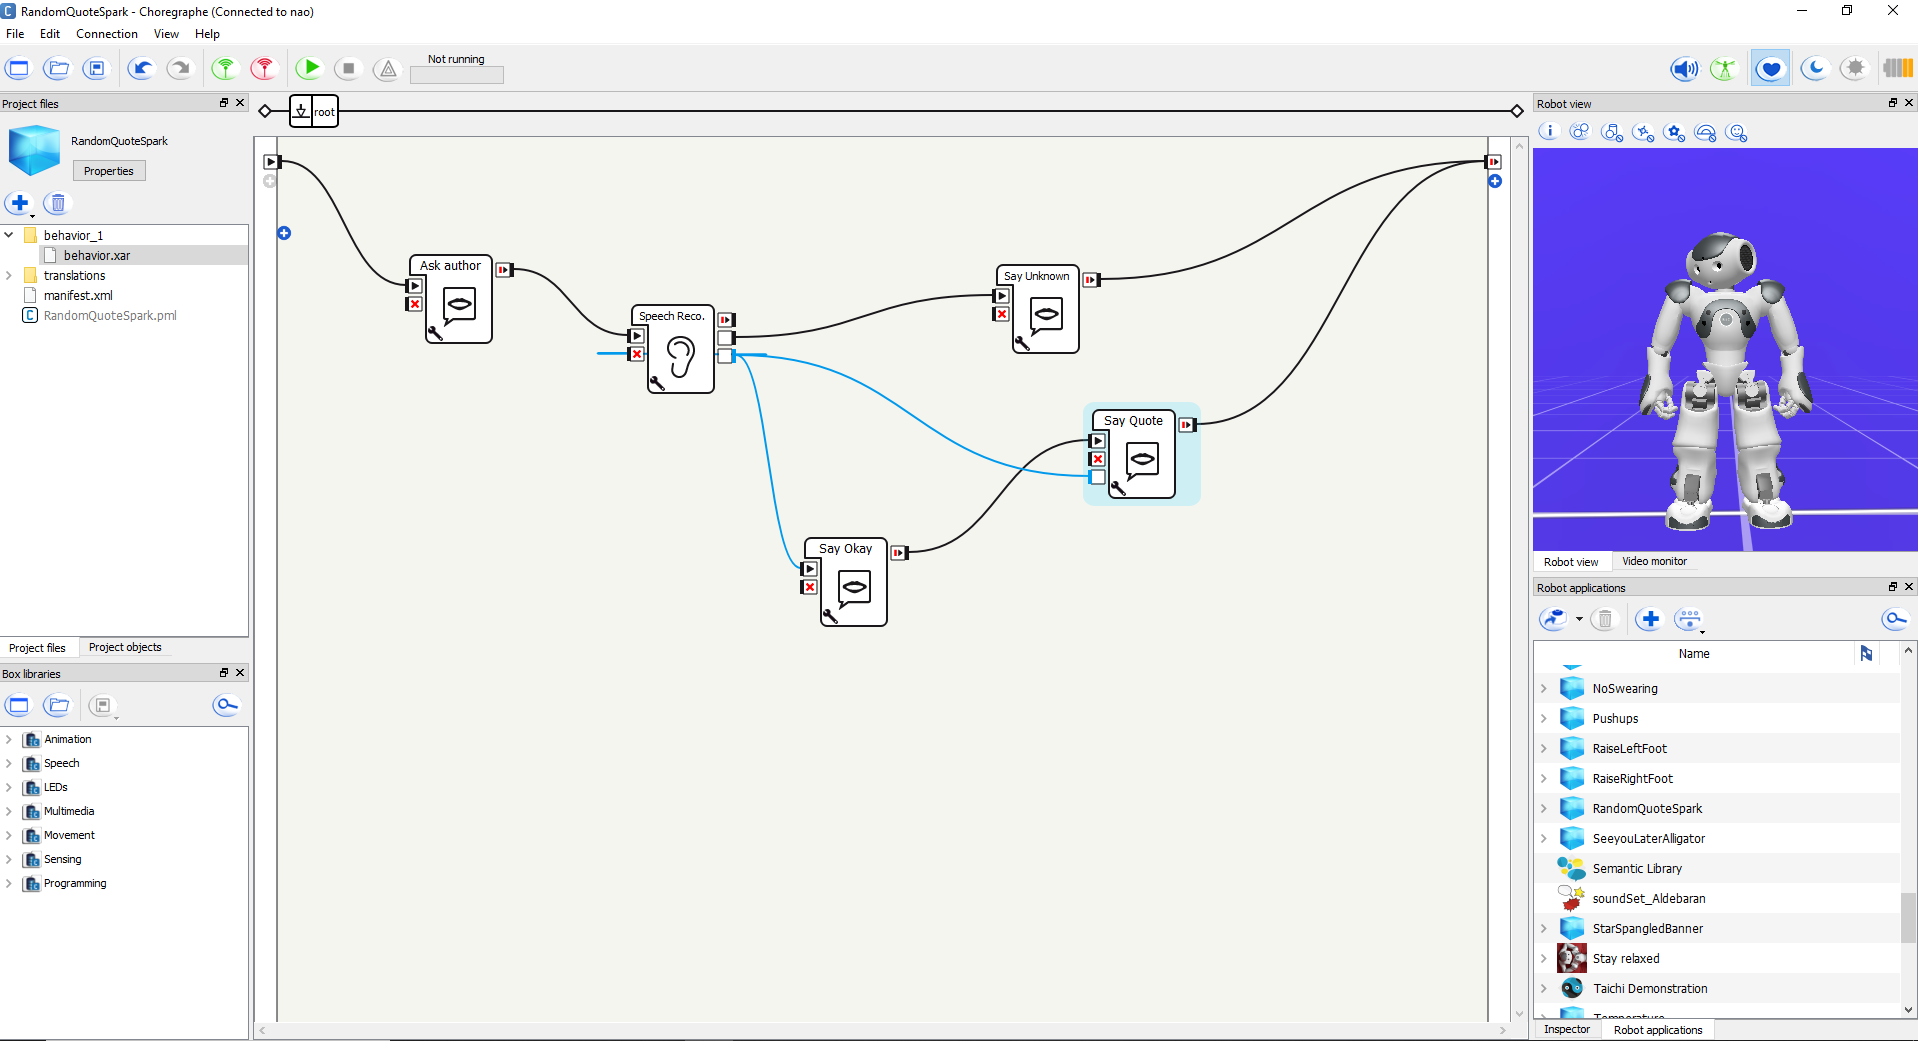
\includegraphics[width =1\linewidth]{robot-spark-proj/screenshot-1.PNG}
    		\caption{Diagram}
    	\end{figure}
    	
    \end{frame}


	\begin{frame}[fragile]{Robot Python2 - Server Request}
		\begin{verbatim}
		# Get request result from spark webserver
		r = requests.get("http://35.226.85.38:80/?author=" + 
		    str(author), timeout=5)
		
		# Convert request to json object
		data = r.json()
	
		# Say quote
		say = str(data['quote']) + ". " + str(data['author'])
		\end{verbatim}
	\end{frame}

\section{Live Demo}

\frame{\sectionpage}
    
    \section{Conclusion and References}
    
    \frame{\sectionpage}
    
    \begin{frame}{Conclusion}
         	\begin{itemize}
         	\item This has been a really fun and great learning experience for our group
         	\pause
         	\item Thank you Professor Calvalcanti for great classes and content.
         	\pause
         \end{itemize}
    \end{frame} 
    
%    \section*{Acknowledgments} %You can remove this if you do not want to use it
%        \begin{frame}{Acknowledgments}
%            The author is extremely thankful to Prof. Antônio F. R. T. Piza for the short, yet wonderful, conversations about this seminar.
%        \end{frame}
    
%    \section*{References} %You can remove this if you do not want to use it
%        \nocite{Djairo} \nocite{PhilPanof} \nocite{Fleming} \nocite{Shankar}
%        \begin{frame}{References}
%            \printbibliography
%        \end{frame}

    \section{}
    \begin{frame}{}
        \centering
            \Huge\bfseries
        \textcolor{orange}{Questions?}
    \end{frame}
\end{document}
